% !TeX root = proyecto.tex

%=========================================================
\chapter{Modelo del alcance}
\label{cap:alcance}

\cdtInstrucciones{
	Indique un resumen que describa el contenido del capítulo.
}
	En este capítulo, exploraremos el objetivo del proyecto, junto con las limitaciones que determinan el alcance del mismo. Añadido a eso definiremos a los usuarios involucrados en el sistema, sus roles y las plataformas compatibles en las que se desarrollará e implementará el proyecto. Nos enfocaremos en identificar las problemáticas clave, desglosando las causas que probablemente las originan y evaluando las consecuencias más probables que podrían surgir si no se abordan adecuadamente.

Asimismo, presentaremos posibles soluciones para cada uno de los problemas detectados, con una síntesis final que propondrá una solución integral capaz de satisfacer la mayor cantidad de requerimientos de los usuarios. Detallaremos los requisitos específicos de los usuarios, ya que serán fundamentales para guiar el diseño y el desarrollo del proyecto en todas sus etapas posteriores, asegurando que se cumplan sus expectativas y necesidades.
%---------------------------------------------------------
\section{Análisis de la problemática}

\cdtInstrucciones{
	Indique en un párrafo o dos el contenido y organización de la problemática.
}
Durante el proceso de migarción al que se ven sometidos los niños inscritos en el PRONIM gran parte de la información necesaria para determinar su nivel educativo se ve retrasada o nunca llega a ser proporcionada al centro de trabajo en el que el niño se va  a incorporar, esto puede ocasionarle un retraso en el desarrollo de las habilidades necesarias para afrontar los retos de su grado escolar aumentando las posibilidades de que el niño abandone su educación.
% - - - - - - - - - - - - - - - - - - - - - - - - - - - - 
\subsection{Contexto del proyecto}

\cdtInstrucciones{
	Indique los antecedentes, contexto y características relevantes necesarios para comprender la problemática a resolver.
}
El PRONIM es un programa gubernamental enfocado en garantizar el acceso a la educación de los niños en condicion migratoria, estas migraciones estan sujetas principalmente aunque no de forma limitada a las oportunidades de trabajo de sus tutores o los propios niños que principalmente estan en la recolección y siembra, por esta razón también es común que los Centro de Trabajo en los que se lleva a cabo la formación del niño no tenga acceso continuo a internet.\\
Actualmente para poder llevar a cabo el seguimiento de los niños se usa el Sistema Nacional de Control Escolar para Migrantes (SINACEM) sin embargo su ultima versión (la versión 2.0) no ha sido concluida desde el año 2011.
% - - - - - - - - - - - - - - - - - - - - - - - - - - - - 
\subsection{Problemas identificados}

\cdtInstrucciones{
	Describa el problema general y realice una lista con los problemas específicos a resolver mediante el proyecto.
}
El problema general que atiende el presente proyecto es: 
La complejidad para mantener un adecuado seguimiento al avance educativo de los niños migrantes.
\begin{quotation}
	{\em ``Descripción de la problemática general''}
\end{quotation}

Los problemas identificados son\FootnotePrioridad

\begin{problemas}
   \problema{P-01}{Detección de un niño que ha comenzado una migración}{Cuando un alumno parte a otro estado en pocas ocasiones la escuela en la que estudiaba es notificada por lo que su partida solo es notada cuando ha pasado un tiempo razonable o por los rumores}{A}
   \problema{P-02}{Evaluación del avance de un alumno}{Debido a la forma en la que se registra el avance de un alumno las evidencias del avance generado por el mismo solo es registrado cada dos meses, si la migración coincide con dichas evaluaciones el avance del alumno queda sin ser registrado de manera apropiada  }{MA}
   \problema{P-03}{Perdida de información de un alumno}{Al realizar una migración existe el riesgo de que documentos importantes se pierdan durante el translado.}{B}
   \problema{P-04}{Duplicidad de alumnos}{Cuando un alumno no es dado de baja en la primera escuela es posible que al terminar el ciclo escolar se intenten generar dos boleta para el mismo niño desde escuelas distintas}{M}
   \problema{P-05}{Falta de comunicación de los CT}{Cada Centro de Trabajo funciona de manera independiente por lo que no hay canales de comunicación que permitan avisar al resto el estado de los alumnos de interes}{MA}
   \problema{P-06}{Detección de necesidades especiales no diagnosticadas}{Un alumno con necesidades especiales no diagnosticadas puede tener problemas para adaptarse a un nuevo ambiente educativo lo que en ultima instancia le repercutira en el aprovechamiento de su educacio, sumado a eso detectar estas posibles necesidades suele representar un reto para el nuevo docente al no conocer del todo al alumno. }{A}
   \problema{P-07}{Deteccion de conductas no deseadas en un alumno}{Tener información de un alumno con conductas no deseadas permite generar nuevas estrategias para mejorar el ambiente en clases, la falta de esta puede ocasionar un retraso no solo en el desarrollo del alumno que tiene las conductas como del resto del grupo.}{M}
   \problema{P-08}{Perdida de fechas de evaluación}{Al realizar una migración existe una posibilidad de que parte de los conocimientos obtenidos por el niño sean mal documentados.}{A}
   \problema{P-09}{Falta de acceso a internet}{La poca cobertura a internet de la que se suele disponer en las zonas de mayor migración dificulta sino es que hasta imposibilita la correcta y rapida trasmisión de información}{B}
\end{problemas}
 
% - - - - - - - - - - - - - - - - - - - - - - - - - - - - 
\subsection{Análisis de causas probables}

\cdtInstrucciones{
	Describa las posibles causas de los problemas señalados.
}
\begin{description}
	\item[P-01A] La falta de tiempo para notificar a la escuela de que el alumno va a darse de baja o a comenzar una migración.
    \item[P-01B] La falta de tiempo para notificar a la escuela de que el alumno va a darse de bajao a comenzar una migración.
	\item[P-01C] Los rumores no son fuentes de información confiable.
 \item[P-02A] Los periodos de evaluación son rigidos y no permiten adaptarse a situaciones como las presentadas por estos niños.
    \item[P-02B] Los profesores no tienen un conducto por medio del cual registrar los avances de los alumnos de forma más fiable que el papel.
	\item[P-02C] El desconocimiento de cuando es necesario realizar la evaluación de un alumno de forma extemporanea.
 \item[P-03A]Las migraciones suelen producirse de manera rapida.
    \item[P-03B] Las migraciones suelen ocurrir de forma desordenada.
	\item[P-03C] No existe un respaldo además de los documentos fisicos.
 \item[P-04A] Los centros de trabajo no tienen una manera de comunicarse para evitar la duplicidad de alumnos.
    \item[P-05A]Todos los centros de trabajo se administran internamente de una forma distinta.
    \item[P-05B] No existen los canales de comuncación adecuados para compartir dicha información.
	\item[P-05C] Algunos centros de trabajo no estan conectados a ninguna red capaz de enviar información a grandes distancias.
 \item[P-06A] Los docentes no necesariamente tienen la formación adecuada para detectar esas necesidades especiales.
    \item[P-06B] Los profesores no tienen un historial completo del comportamiento del alumno.
	\item[P-06C] En caso de que un docente anterior haya detectado esas necesidades al cambiar de escuela esos registros se pierden.
 \item[P-07A] Los docentes no necesariamente tienen la formación adecuada para detectar esos transtornos de conducta.
    \item[P-07B] Los profesores no tienen un historial completo del comportamiento del alumno.
	\item[P-07C] En caso de que un docente anterior haya detectado esos comportamientos al cambiar de escuela esos registros se pierden.
 \item[P-08A] Los periodos de evaluación son rigidos y no permiten adaptarse a situaciones como las presentadas por estos niños.
    \item[P-08B] No existe un seguimiento activo del avance de cada alumno guardado en un lugar de facil acceso para futuros profesores.
	\item[P-08C] Es imposible para el profesor anterior entregar la calificación obtenida por el alumno a su siguiente profesor.
 \item[P-09A] La localización de los centros de trabajo suele ser zonas de bajos recursos.
    \item[P-09B] Desconocimiento de los ciminetos necesarios para el uso de internet .
	\item[P-09C] Falta de dinero para generar una conexión a interneto a otros servicios necesarios.
\end{description}


% - - - - - - - - - - - - - - - - - - - - - - - - - - - - 
\subsection{Análisis de posibles consecuencias}
La poca cobertura a internet de la que se suele disponer en las zonas de mayor migración dificulta sino es que hasta imposibilita la correcta y rapida trasmisión de información
\cdtInstrucciones{
	Describa las consecuencias inmediatas, a mediano y largo plazo si la problemática persiste.
}
\begin{description}

	\item[P-01A] El programa contabiliza y atiende menos niños de los que realmente son por lo que se le asigna menos dinero del que requiere.
	\item[P-01B] Los alumnos migrantes que no estan registrados en el PRONIM tiene màs probabilidades de dejar los estudios.
     \item[P-01C] La cifra de alumnos que dejan la escuela esta inflada.
     \item[P-02A] Al perder una evaluaciòn un niño migrante tiene mayor probabilidad de perder el año escolar.
	\item[P-02B] Aumenta la probabilidad de tener problemas para entender nuevos temas si no se detecta a tiempo que el alumno no a comprendido cierto tema.
     \item[P-02C] Alumnos migrantes con alguna clase de apoyo economico por promedio aumentan sus posibilidades de perderlo.
     \item[P-02D] Si algùn alumno necesita de esos apoyos y los pierde sus posibilidades de dejar la escuela aumenta.
     \item[P-03A] Al perder informaciòn se le dificulta al alumno acceder a nuevos niveles educativos.
	\item[P-03B] Cuando un alumno pierde informaciòn dificulta al alumno acceder a apoyos economicos.
     \item[P-03C] Cuando se pierde la informaciòn de un alumno se le dificulta la posibilidad de acceder a los servicios de salud.
     \item[P-03D] Cuando un alumno pierde su informaciòn dificulta la posibilidad de identificarlo en caso de un accidente.
     \item[P-04A] Resolver la duplicidad genera un aumento en los gastos administrativos derivados.
    \item[P-04B] En caso de no resolver la duplicidad aumenta el costo al expedir dos boletas en lugar de una.
    \item[P-05A] Debido a la falta de comunicaciòn los alumnos aumentan su probabilidad de perder evaluaciones.
	\item[P-05B] Si un alumno tiene necesidades especiales no diagnosticadas pero si identificadas no es posible que sus proximos profesores lo conozcan.
    \item[P-05C] Si un alumno tiene comportamientos peligrosos identificados no es posible que sus proximos profesores lo conozcan.
    \item[P-05A] Debido a la falta de comunicaciòn los alumnos aumentan su probabilidad de perder evaluaciones.
	\item[P-05B] Si un alumno tiene necesidades especiales no diagnosticadas pero si identificadas no es posible que sus proximos profesores lo conozcan.
    \item[P-05C] Si un alumno tiene comportamientos peligrosos identificados no es posible que sus proximos profesores lo conozcan.
    \item[P-06A] Que un alumno no obtenga la ayuda necesaria aumenta la posibilidad de que pierda el año.
	\item[P-06B] Si un alumno tiene necesidades especiales no diagnosticadas y no obtiene la ayuda que necesita sus posibilidades de dejar la escuela se ven aumentadas.
    \item[P-06C] Si un alumno tiene necesidades especiales y no obtiene la ayuda este tiene una mayor probabilidas de sufrir de bullying.
    \item[P-07A] Que un alumno no obtenga la ayuda necesaria aumenta la posibilidad de que pierda el año.
	\item[P-07B] Si un alumno tiene comportamientos peligrosos no obtiene la atenciòn necesaria sus posibilidades de dejar la escuela se ven aumentadas.
    \item[P-07C] Si un alumno tiene comportamientos peligrosos y no es atendido este tiene una mayor probabilidas de hacer bullying a sus compañeros .
    \item[P-09A] El poco acceso a internet dificulta respaldar su informaciòn.
	\item[P-09B] El poco acceso a internet dificulta su acceso a .
    \item[P-09C] Si un alumno tiene comportamientos peligrosos y no es atendido este tiene una mayor probabilidas de hacer bullying a sus compañeros .
\end{description}
 
% - - - - - - - - - - - - - - - - - - - - - - - - - - - - 
\subsection{Características de la solución}

\cdtInstrucciones{
}

Para atender la problemática anterior se propone implementar las siguientes acciones.

\begin{description}
	\item[P-01]	Identificar al alumno con un id único creado con datos personales, que al registrarse de nuevo en otro centro pronim sea detectado al instante y se le pueda dar seguimiento, al igual que después de que el profesor notifique que ha faltado varias veces seguidas se notificará para que suba las calificaciones del alumno y se pueda dar seguimiento.
	\item[P-02] la sección de subir calificaciones estará permanentemente abierta para el registro de calificaciones de los alumnos que se identificó migrando, al ser identificados por faltas o por registro del mismo en otro centro, se notificará al profesor de subir las calificaciones de ese alumno cada tercer día de no subirlas en una semana, se notificara a un superior encargado del profesor (director) para darle seguimiento.
         \item[P-03] Al identificar al alumno en otro centro PRONIM y poder retroalimentar su avance, solo se genera la boleta de la última institución en la que se encontró inscrito.


         \item[P-04]Se registrará cada centro de trabajo y se podra ver el estado actual de cada alumno dentro de cada centro así como su identificación por ID único al registrarlo dos veces y dar la opción de la baja de un centro y retroalimentar al nuevo centro con los últimos datos registrados.
         \item[P-05] Cada profesor podrá tener anotaciones del alumno seccionadas por tipo de nota prara abarcar desde su forma de aprendizaje hasta si tiene alguna condición especial y el nuevo profesor tenga más información del alumno.

         \item[P-06] Al igual que con las necesidades especiales con las nota del alumno se tendrá un registro de las conductas no seseadas y se podrá terner algo de comunicación del profesor que ya estuvo con el alumno para el nuevo profesor.

         \item[P-07]  El profesor será notificado en el momento en el que se identifique una migración por parte del alumno, y se seguirá notificando cada 3 días hasta que suba las calificaciones del niño o pase una semana y se notifique al director para darle seguimiento. 

         \item[P-08]
\end{description}

% - - - - - - - - - - - - - - - - - - - - - - - - - - - - 
\subsection{Síntesis de la problemática}

\cdtInstrucciones{
	Redacte las conclusiones del análisis de la problemática. Explique de manera general la solución o sistema a realizar a manera de propuesta y los beneficios que se obtendrán al implementar la solución.
}

%---------------------------------------------------------
\section{Objetivos del proyecto}

% - - - - - - - - - - - - - - - - - - - - - - - - - - - - 
\subsection{Objetivo general}

\cdtInstrucciones{
	Redacte el objetivo general del proyecto de la forma:\\
	VERBO EN INFINITIVO + (LO QUE SE VA A REALIZAR CON 2 O 3 CARACTERÍSTICAS RELEVANTES) + ``para'' + PROBLEMA QUE RESUELVE + ``mediante'' + 2 O 3 CARACTERÍSTICAS RELEVANTES DE LA SOLUCIÓN.
}

\begin{quotation}
	{\em ``Objetivo''}
\end{quotation}

% - - - - - - - - - - - - - - - - - - - - - - - - - - - - 
\subsection{Objetivos específicos}

\cdtInstrucciones{
	Liste los objetivos específicos adoptando el enfoque que más se adapte a su proyecto: por etapas, de lo general a lo específico, señalando componentes o partes de la solución, etc.
}

\begin{itemize}
	\item...
\end{itemize}


%---------------------------------------------------------
\section{Usuarios identificados}

\cdtInstrucciones{
	Coloque un diagrama a manera de organigrama en donde se indiquen quienes serán usuarios del sistema. 
}

\begin{figure}[htbp!]
	\begin{center}
		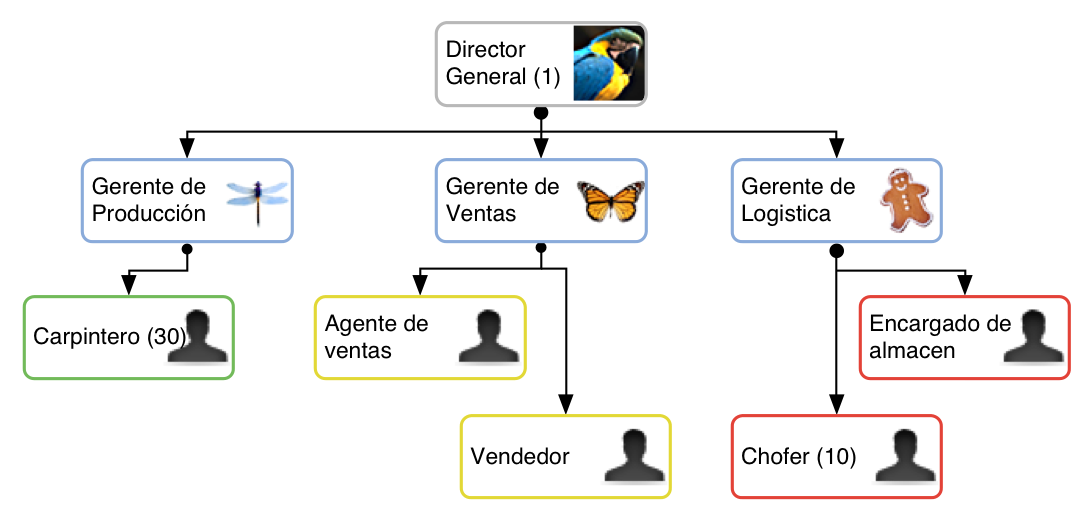
\includegraphics[width=.8\textwidth]{images/organigramaEm}
		\caption{Organigrama de la Mueblería Qetzal S. A. de C. V.}
		\label{fig:organigrama}
	\end{center}
\end{figure}


%---------------------------------------------------------
\section{Procesos involucrados}

\cdtInstrucciones{
	Coloque el mapa de procesos de la organización y liste a continuación los proceso que serán afectados por el desarrollo del sistema. Para cada proceso indique: Clave, Nombre y descripción.
}

\begin{figure}[htbp!]
	\begin{center}
		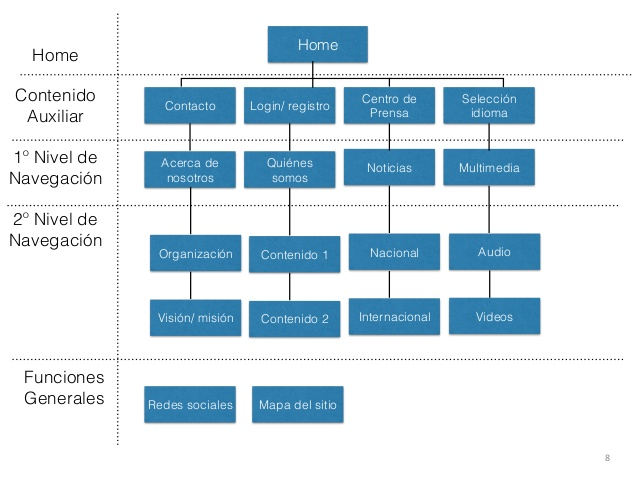
\includegraphics[width=.8\textwidth]{images/mapa}
		\caption{Mapa de procesos de la Mueblería Qetzal S. A. de C. V.}
		\label{fig:mapaProcASIS}
	\end{center}
\end{figure}

\begin{description}
	\item[PR-01] Nombre del proceso. Descripción del proceso.
\end{description}

%---------------------------------------------------------
\section{Requerimientos de usuario}

\cdtInstrucciones{
	Identifique y describa los requerimientos del usuario señalando: id, nombre, descripción y prioridad.
}

Los requerimientos del usuario son los siguientes\FootnoteStatus:

\begin{requerimientosU}
	\FRitem{RU-01}{Nombre del requerimiento}{Descripción del requerimiento.}{1}{\TODO}
	\FRitem{}{...}{...}{...}{...}
\end{requerimientosU}
\begin{table}[htbp]
\centering
\begin{tabular}{|c|l|p{10cm}|}
\hline
\textbf{ID} & \textbf{Nombre del Requerimiento} & \textbf{Descripción} \\ \hline
RNF1 & Seguridad básica de la Información & El sistema debe proteger los datos de los estudiantes y profesores mediante contraseñas y permisos de acceso por roles, implementando autenticación básica. \\ \hline
RNF2 & Disponibilidad del Sistema & El sistema debe estar disponible en horarios escolares y accesible de forma remota para los profesores y directores, con un tiempo de actividad mínimo del 90\%. \\ \hline
RNF3 & Tiempo de Respuesta & Las operaciones principales del sistema, como la consulta de información o actualización de datos, deben tener un tiempo de respuesta inferior a 3 segundos en entornos controlados de prueba. \\ \hline
RNF4 & Accesibilidad & El sistema debe cumplir con estándares de accesibilidad web (como WCAG 2.0), garantizando que los profesores y directores con discapacidades visuales o auditivas puedan usarlo sin dificultades. \\ \hline
RNF5 & Facilidad de mantenimiento & El sistema debe estar bien documentado para que otros estudiantes o profesores puedan mantenerlo y hacer mejoras sin dificultad. \\ \hline
RNF6 & Compatibilidad multiplataforma & El sistema debe ser accesible desde navegadores web comunes como Chrome o Firefox, y no requerir software adicional más allá de un navegador. \\ \hline
RNF7 & Interfaz amigable para usuarios & El sistema debe tener una interfaz sencilla y fácil de usar, con formularios claros y navegación intuitiva para profesores con poca experiencia técnica. \\ \hline
RNF8 & Copia de seguridad manual & El sistema debe permitir realizar copias de seguridad manuales de los datos educativos, exportando archivos en formatos como CSV o Excel para garantizar la conservación de la información. \\ \hline
RNF9 & Bajo costo de implementación & El sistema debe usar tecnologías y recursos gratuitos o de bajo costo para mantenerse dentro del presupuesto del proyecto. \\ \hline
RNF10 & Requerimientos técnicos mínimos & El sistema debe funcionar en computadoras con especificaciones mínimas (procesadores dual-core, 4GB de RAM, etc.), lo que lo hace viable para centros educativos con recursos limitados. \\ \hline
\end{tabular}
\caption{Requerimientos no funcionales para el sistema}
\end{table}
%---------------------------------------------------------
\section{Especificación de plataforma}	

\cdtInstrucciones{
	Coloque un diagrama y su descripción para aclarar el tipo de solución propuesta. \\
	
 En esta sección se debe aclarar:
	
\begin{description}
	\item[Tipo de sistema:] Web, aplicación móvil, de escritorio, híbrida, etc.
	\item[Software requerido:] Programas que se deberán instalar, desde el sistema operativo, compiladores, interpretes, servidores, etc.
	\item[Hardware requerido:] CPU, núcleos, velocidad, memoria, disco duro, etc.
	\item[servicios:] De conexión, seguridad, firewall, respaldo de energía, redundancia, uso de raids, etc.
\end{description}
}

\begin{figure}[htbp!]
	\begin{center}
		\fbox{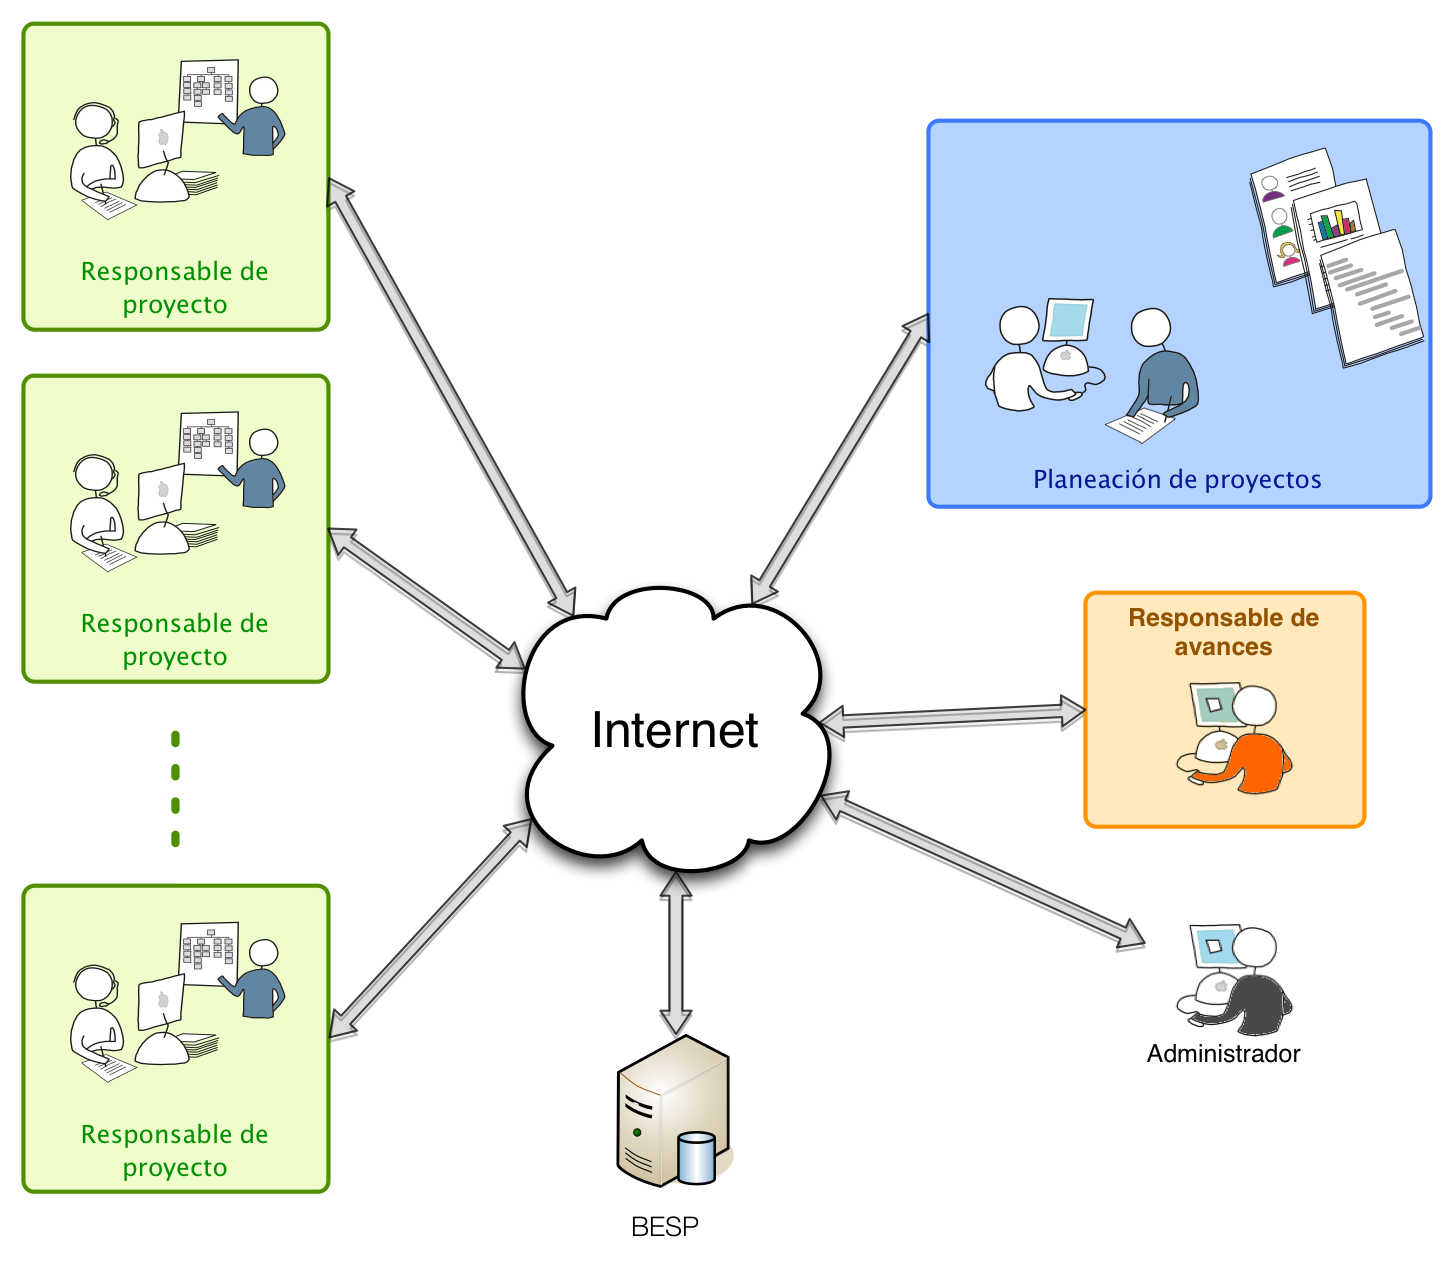
\includegraphics[width=.6\textwidth]{images/arquitectura}}
		\caption{Arquitectura del sistema.}
		\label{fig:arquitectura}
	\end{center}
\end{figure}

En la figura~\ref{fig:arquitectura} se describe la estructura del sistema, en ella se detalla ...


